\section{Elimination of nondeterminism}

Every non-deterministic finite automaton can always be transformed into an equivalent deterministic one. 
Consequently, every right linear grammar always admits an equivalent non-ambiguous right linear one. 
Thus, every ambiguous regular expression can always be transformed into a non-ambiguous one. 
The algorithm to transform a non-deterministic automaton into a deterministic one is structured in two phases: 
\begin{enumerate}
    \item Elimination of the spontaneous moves. As such moves correspond to copy rules, it suffices to apply the algorithm for removing the copy rules. 
    \item Replacement of the non-deterministic multiple transitions by changing the automaton state set. This is the well known subset construction. 
\end{enumerate}
\begin{example}
    Given the following automaton: 
    \begin{figure}[H]
        \centering
        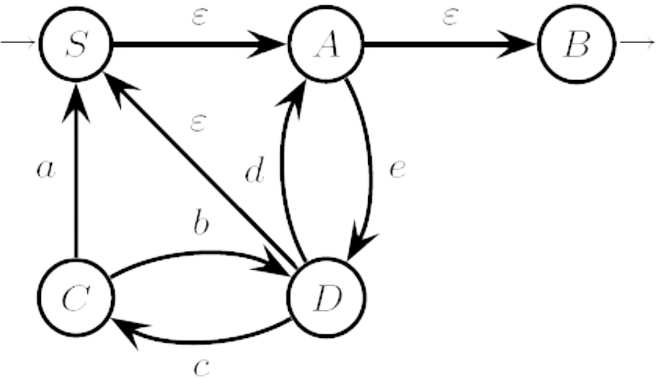
\includegraphics[width=0.25\linewidth]{images/oaut.png}
    \end{figure}
    After applying the algorithm we have: 
    \begin{figure}[H]
        \centering
        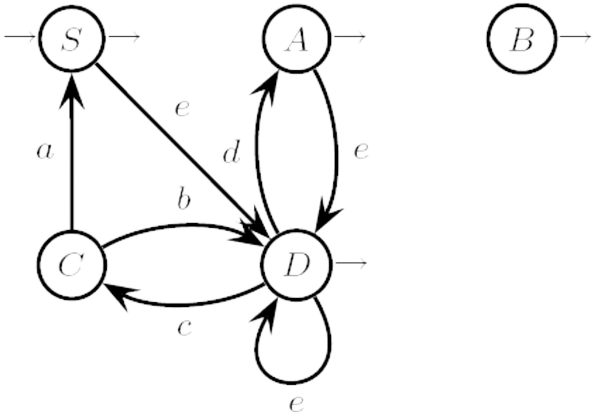
\includegraphics[width=0.25\linewidth]{images/faut.png}
    \end{figure}
    If after eliminating all the $\varepsilon$-arc the automaton is still non-deterministic, then go to the second phase.
\end{example}